% Figure 3: what is validated, on which silicon, and what is not.
%
% Build: tectonic docs/figures/fig3_status.tex
%
% Filled means it ran on that GPU and passed its gate. Nothing is marked
% done on hardware it has never run on. Sources are the session entries in
% journal/u2-hopper-design.md and the artifacts under journal/remote/.

\documentclass[border=14pt]{standalone}
% Shared style for all Inkling-turbo figures.
% Included by each standalone figure so they read as one family.
\usepackage{tikz}
\usepackage{pgfplots}
\pgfplotsset{compat=1.18}
\usetikzlibrary{calc,plotmarks,backgrounds}

% palette
\definecolor{ours}{HTML}{0B6E6A}     % our kernel
\definecolor{floorc}{HTML}{64748B}   % the biasless floor
\definecolor{prod}{HTML}{C2410C}     % the path vLLM ships
\definecolor{altA}{HTML}{9A3412}     % other day-0 paths
\definecolor{altB}{HTML}{78350F}
\definecolor{ink}{HTML}{111827}      % text
\definecolor{guide}{HTML}{DDE1E6}    % grid
\definecolor{band}{HTML}{F4F6F8}     % group banding
\definecolor{okc}{HTML}{15803D}      % validated
\definecolor{partc}{HTML}{B45309}    % partial

% shared axis look: no frame, no ticks, faint grid, small labels
\pgfplotsset{
  inkling/.style={
    scale only axis,
    axis line style={draw=none},
    tick style={draw=none},
    grid style={line width=0.45pt, color=guide},
    xticklabel style={font=\scriptsize, color=ink!62},
    yticklabel style={font=\scriptsize, color=ink!88},
    xlabel style={font=\footnotesize, color=ink!85},
    ylabel style={font=\footnotesize, color=ink!85},
    clip=false,
  },
}

% figure title + standfirst, placed above a named axis
\newcommand{\figtitle}[3]{%
  % #1 axis name, #2 title, #3 standfirst
  \node[anchor=north west, font=\bfseries, color=ink]
    at ($(#1.north west)+(\titleoffset,\titletop)$) {\large #2};
  \node[anchor=north west, font=\scriptsize, color=ink!58,
        text width=\standfirstwidth]
    at ($(#1.north west)+(\titleoffset,\titlesub)$) {#3};
}


\begin{document}
\sffamily
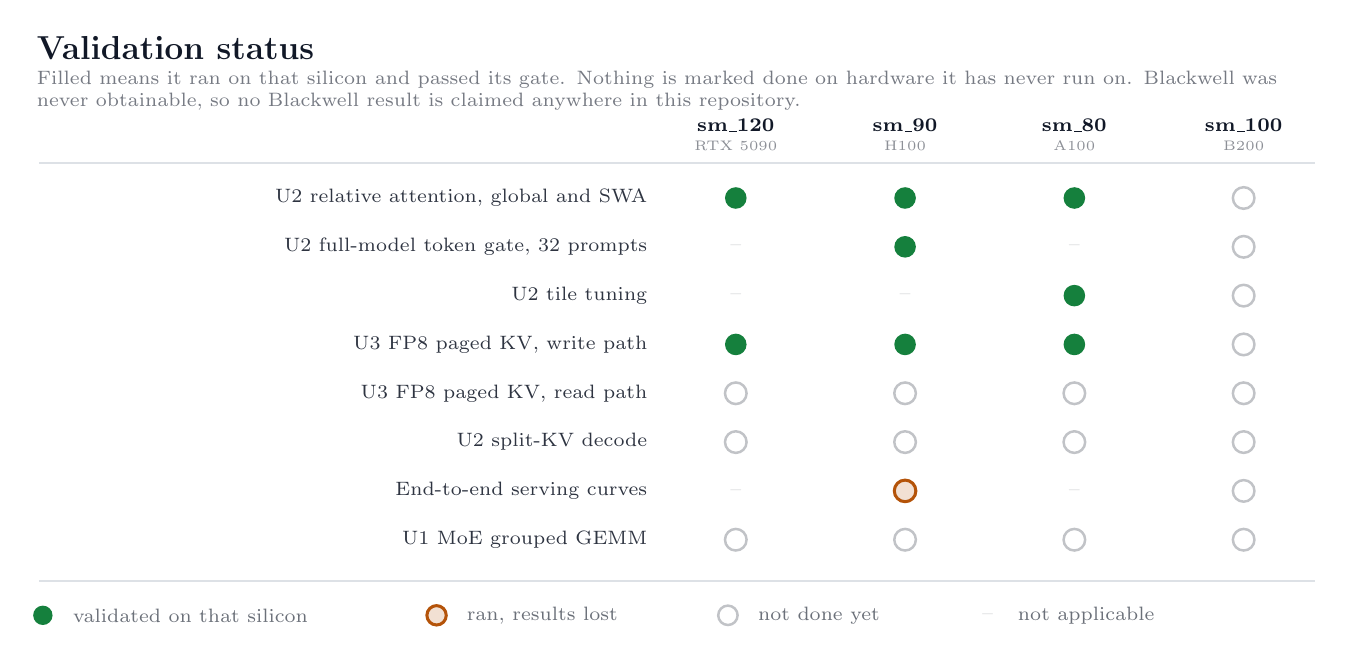
\begin{tikzpicture}[font=\sffamily]

\def\cz{9.0}      % x of first architecture column
\def\cw{2.15}     % column pitch
\def\rh{0.62}     % row pitch
\def\labx{8.0}    % right edge of the row labels
\def\rulel{0.15}  % rules
\def\ruler{16.35}

\node[anchor=north west, font=\bfseries, color=ink] at (0,1.05cm)
  {\large Validation status};
\node[anchor=north west, font=\scriptsize, color=ink!58, text width=16.2cm]
  at (0,0.62cm)
  {Filled means it ran on that silicon and passed its gate. Nothing is marked
   done on hardware it has never run on. Blackwell was never obtainable, so
   no Blackwell result is claimed anywhere in this repository.};

% ---- column headers
\node[font=\scriptsize\bfseries, color=ink] at (9.00cm,-0.20cm) {sm\_120};
\node[font=\tiny, color=ink!48]             at (9.00cm,-0.46cm) {RTX 5090};
\node[font=\scriptsize\bfseries, color=ink] at (11.15cm,-0.20cm) {sm\_90};
\node[font=\tiny, color=ink!48]             at (11.15cm,-0.46cm) {H100};
\node[font=\scriptsize\bfseries, color=ink] at (13.30cm,-0.20cm) {sm\_80};
\node[font=\tiny, color=ink!48]             at (13.30cm,-0.46cm) {A100};
\node[font=\scriptsize\bfseries, color=ink] at (15.45cm,-0.20cm) {sm\_100};
\node[font=\tiny, color=ink!48]             at (15.45cm,-0.46cm) {B200};

\draw[guide, line width=0.7pt] (\rulel cm,-0.68cm) -- (\ruler cm,-0.68cm);

% state codes: 1 validated, 2 ran but results lost, 3 not done, 4 not applicable
\foreach \r/\name/\a/\b/\c/\d in {%
  0/{U2 relative attention, global and SWA}/1/1/1/3,
  1/{U2 full-model token gate, 32 prompts}/4/1/4/3,
  2/{U2 tile tuning}/4/4/1/3,
  3/{U3 FP8 paged KV, write path}/1/1/1/3,
  4/{U3 FP8 paged KV, read path}/3/3/3/3,
  5/{U2 split-KV decode}/3/3/3/3,
  6/{End-to-end serving curves}/4/2/4/3,
  7/{U1 MoE grouped GEMM}/3/3/3/3%
}{
  \pgfmathsetmacro{\ry}{-1.12-\r*\rh}
  \node[anchor=east, font=\scriptsize, color=ink!88] at (\labx cm,\ry cm)
    {\name};
  \foreach \ci/\st in {0/\a, 1/\b, 2/\c, 3/\d}{
    \pgfmathsetmacro{\xx}{\cz+\ci*\cw}
    \ifnum\st=1
      \node[circle, fill=okc, minimum size=7.8pt, inner sep=0]
        at (\xx cm,\ry cm) {};
    \fi
    \ifnum\st=2
      \node[circle, draw=partc, fill=partc!18, line width=1.1pt,
            minimum size=7.8pt, inner sep=0] at (\xx cm,\ry cm) {};
    \fi
    \ifnum\st=3
      \node[circle, draw=ink!26, line width=0.9pt, minimum size=7.8pt,
            inner sep=0] at (\xx cm,\ry cm) {};
    \fi
    \ifnum\st=4
      \node[font=\scriptsize, color=ink!22] at (\xx cm,\ry cm) {--};
    \fi
  }
}

\draw[guide, line width=0.7pt]
  (\rulel cm,-5.98cm) -- (\ruler cm,-5.98cm);

% ---- legend
\begin{scope}[shift={(0.2cm,-6.42cm)}]
  \node[circle, fill=okc, minimum size=7pt, inner sep=0] at (0,0) {};
  \node[anchor=west, font=\scriptsize, color=ink!62] at (0.26cm,0)
    {validated on that silicon};
  \node[circle, draw=partc, fill=partc!18, line width=1.1pt, minimum size=7pt,
        inner sep=0] at (5.0cm,0) {};
  \node[anchor=west, font=\scriptsize, color=ink!62] at (5.26cm,0)
    {ran, results lost};
  \node[circle, draw=ink!26, line width=0.9pt, minimum size=7pt, inner sep=0]
    at (8.7cm,0) {};
  \node[anchor=west, font=\scriptsize, color=ink!62] at (8.96cm,0)
    {not done yet};
  \node[font=\scriptsize, color=ink!22] at (12.0cm,0) {--};
  \node[anchor=west, font=\scriptsize, color=ink!62] at (12.26cm,0)
    {not applicable};
\end{scope}

\end{tikzpicture}
\end{document}
